\documentclass{article}
\usepackage{graphicx}
\usepackage{amsmath}
\begin{document}
\title{\vspace*{5cm}\hrule~\\ QeCode User Manual\\~\\
\small Manual v0.3.0a documenting QeCode v2.1.0a\\~\hrule} % QeCode Anniversary Edition ! 
\author{Marco Benedetti, Arnaud Lallouet, J\'er\'emie Vautard\vspace*{2mm}\\ 
University of Orl\'eans - LIFO\vspace*{2mm}}
\date{\small\today}
\maketitle
\thispagestyle{empty}
\subsection*{Manual revisions}
\begin{itemize}
\item v0.3.0a: Heavy code refactoring after more than a decade. Some sections reformulated in proper english thanks to Guy-Paul-Theo the Fourth. 
\item v0.2.1: class names changes in last version of QeCode.
\item v0.2: documenting Qecode2, introducing QCOP+.
\item v0.1.2: improves QCSP$^+$ introduction, full source code of the example.
\item v0.1.1: overview, how to declare a QCSP$^+$ formula, how to post constraints, a simple example.
\end{itemize}
\newpage

\section{Before you start}
QeCode is a comprehensive C++ library specifically designed for formulating and resolving Quantified Constraint Satisfaction Problems (QCSP) and Quantified Constraint Optimization Problems (QCOP). It introduces an advanced modeling language featuring {\em restricted quantification}, building upon the robust finite domain constraint solving capabilities of the GeCode library \cite{gecode}.

This manual presupposes successful compilation of QeCode and its accompanying examples. For compilation instructions, refer to the QeCode website or the "COMPILING" document within the examples directory. While this guide provides a basic overview of Quantified CSP (including $QCSP^+$), its primary goal is not to delve into the intricacies of quantified problem modeling, but to facilitate a swift and efficient start with QeCode.

Prior knowledge of finite domain constraint programming and foundational C++ skills are recommended for the users of this guide.

\section{A Quick Overview of $QCSP^+$ and $QCOP^+$}
\subsection{QCSP$^+$}
In essence, solving a Constraint Satisfaction Problem (CSP) revolves around the question: "Is there an assignment for all variables in the problem that satisfies all constraints?" For a CSP comprising $n$ variables and $m$ constraints, this can be represented logically as: 
$$\exists x_1 \exists x_2 \ldots \exists x_n~~.~~c_1 \wedge c_2 \wedge \ldots \wedge c_m $$

\noindent The $QCSP^+$ framework extends this concept to model problems in the form:
\begin{align*}
    &Q_1 ~ x_1 ~ [C_1]\\
    ~~&Q_2 ~ x_2 ~ [C_2]\\
    ~~~~&\ldots\\
    ~~~~~~&Q_n ~ x_n ~ [C_n]\\
    ~~~~~~~~G\\
\end{align*}
where $Q_i$ is a quantifier (either $\exists$ or $\forall$) for $i \in [1..n]$, and $x_i$ represents a set of finite domain variables. $C_i$ is a CSP limiting the values of the variables defined earlier to those consistent with the constraints. This construct, $Q_i ~ x_i ~ [C_i]$, is termed a {\em restricted quantified set of variables} or {\em rqset}. The final CSP, $G$, referred to as the {\em goal}, must be satisfied by any assignment adhering to the preceding rqsets. The bracket notation for $C_i$ implies a condition of "such that," linking the rqset to the rest of the formula with $\wedge$ if $Q_i$ is $\exists$ and with $\rightarrow$ if $Q_i$ is $\forall$. For instance, the formula: 
$$\exists x \forall y [x \neq y] \exists z [z < x] . z < y$$ 
is logically interpreted as: 
$$\exists x \forall y . (x \neq y) \rightarrow \exists z . (z < x) \wedge (z < y)$$ 
Further technical details on $QCSP^+$ can be found in \cite{10.5555/1625275.1625280}.

The original $QCSP$ framework \cite{10.1007/3-540-46135-3_25} did not include restricted quantifiers. $QCSP^+$ was developed to better model scenarios such as games where a player's moves depend on preceding actions. Consider two games, the Nim game and its variant "Nim-Fibonacci": 

In the Nim game, players alternate taking 1 to 3 matches from a pile of $n$ matches. The player who picks the last match wins. The first player's winning strategy in classical $QCSP$ can be modeled as:
$$\exists x_1 \in [1..3] \forall y_1 \in [1..3] \ldots \exists x_{n/4} ~~~~ (\sum_{i=1}^{n/4} x_i + y_i = n)$$

In Nim-Fibonacci, the first player takes any number of matches (but not all), and each subsequent player can take up to double what their opponent took previously. The number of matches a player can take varies, making it impossible to predict in advance. In $QCSP^+$, this scenario is naturally represented:

\begin{align*}
    &\exists x_1 \in [1.. n-1]\\
    &\forall y_1 \in [1..n-1] ~(y_1\leq 2x_1) \wedge (x_1+y_1 \leq n) ~ \rightarrow \\
    &\exists x_2 \in [1..n-1] ~ (x_2\leq2y_1) \wedge (x_1+y_1+x_2 \leq n)  ~ \wedge \\
    &\hspace{3mm}\vdots\\
    &\top
\end{align*}

In this particular example, the objective of the game is encapsulated by the constraints $(x_1+y_1+\ldots \leq n)$. If one player empties the set, their opponent cannot move, thereby losing the game. Consequently, the goal is redundant in this instance and is set to true.


\subsection{QCOP$^+$}
QCOP$^+$ represents an evolution of QCSP$^+$, introducing optimization conditions at each existential scope. In these problems, each existential scope corresponds to a different player, each aiming to optimize their own parameters. The first player sets their variables based on their optimization goals, considering that the subsequent player will respond according to their own criteria, and so forth.

\begin{figure}[b]
\centerline{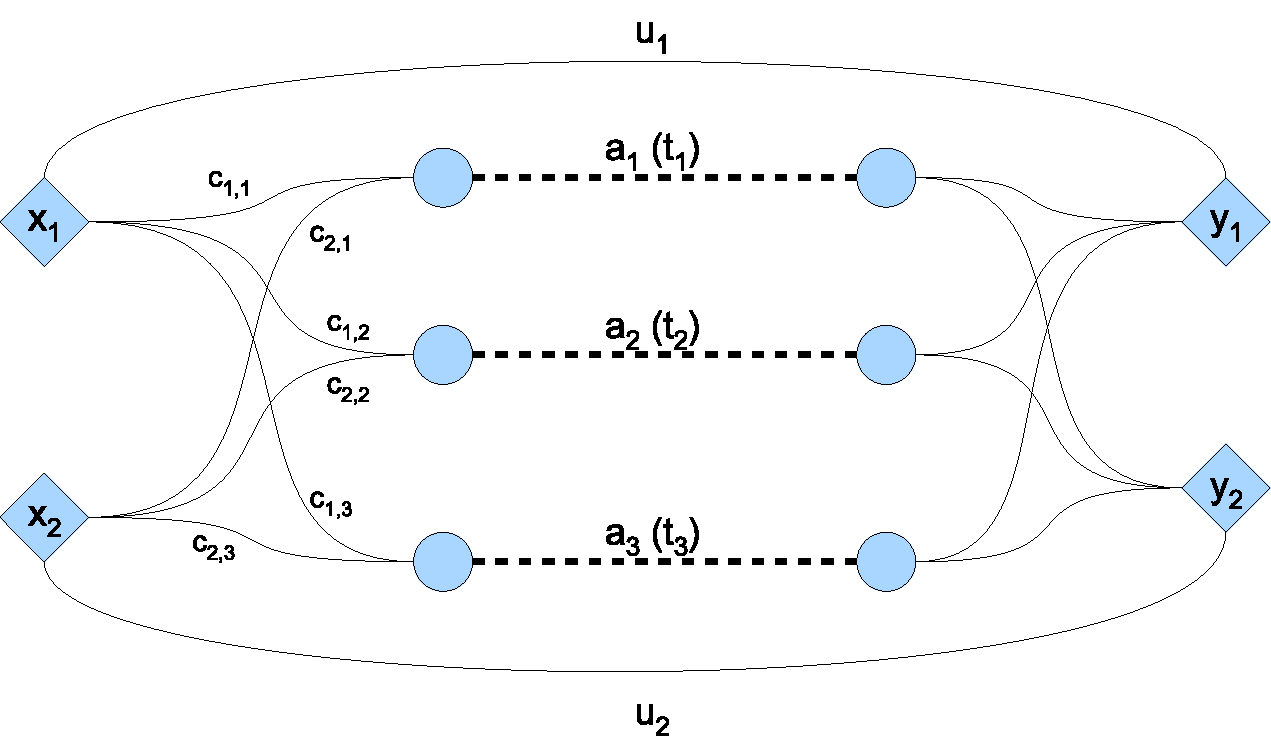
\includegraphics[height=4cm]{network.pdf}}
\caption{A network pricing problem.} \label{fig-network}
\end{figure}

Consider, for example, a network pricing problem: this involves setting tariffs on network links to maximize the profits of the link owner (the leader). As illustrated in Figure \ref{fig-network}, the network includes $NCustomer$ customers (the followers), each routing their data independently at the lowest cost. Customer $i$ aims to transmit $d_i$ units of data from a source $x_i$ to a target $y_i$. Each path from a source to a target crosses a tolled arc $a_j$, incurring a cost $c_{ij}$ on the links owned by other providers between $s_i$ and $a_j$. It is assumed that each customer $i$ seeks to minimize the data routing cost, with the option to choose another provider at a cost $u_i$. The objective is to determine the toll $t_j$ for crossing each tolled arc $a_j$, maximizing the telecom operator's revenue. In the depicted scenario (Figure \ref{fig-network}), there are 2 customers and 3 tolled arcs. This problem can be formulated as a QCOP:

{\small
\begin{verbatim}
const NCustomer
const NArc
const c[NCustomer,NArc] // c[i,j]: fixed cost for Ci to reach Aj
const d[NCustomer]      // d[i]: demand for customer i
const u[NCustomer]      // u[i]: maximum price for customer i
\exists t[1], ..., t[NArc] in [0,max]
|  \forall k in [1,NCustomer]
|  |  \exists a in [1,NArc],
|  |  |     cost in [1,max], 
|  |  |     income in [0,max]
|  |  |  cost = (c[k,a]+t[a])*d[k]
|  |  |  income = t[a]*d[k]
|  |  |  cost <= u[k]
|  |  minimize(cost)
|  s:sum(income)
maximize(s)
\end{verbatim}
}

The optimization aspect is encapsulated in the last three lines. Excluding these lines transforms the expression into a standard QCSP$^+$ problem.

\section{Problem Modeling and Solving}

The declaration of a $QCSP^+$ problem in QeCode consists in declaring: 
\begin{enumerate}
\item how many rqsets the problem contains, and for each one, its number of variables
\item For each rqset : 
\begin{itemize}
\item the domain of each of its variables
\item its constraints
\end{itemize} 
\item the constraints of the goal. 
\end{enumerate}
QeCode provides a set of methods which allows to perform each of these steps in the order they are described. 

 
\subsection{Headers and preliminary definitions}
Let us write the code that solves the  $QCSP^+$ corresponding to the network pricing example given above (without considering the optimization part), with 2 clients, and 3 links.

Qecode is a C++ library that you have to link against. To use this library, here are the different headers you need to include: 
\begin{itemize}
\item {\tt QProblem.h} contains all the necessary to create quantified problems. This header indirectly the Gecode minimodel file which is needed to post the most common constraints. 
\item {\tt qsolver\_qcop.hh} contains the solver class.
\end{itemize}
These two files have to be included for modeling and solving the example above.  An object of the class {\tt QProblem} represents a $QCSP^+$ problem. The only public constructor must be given several parameters: 
\begin{itemize}
\item the number of rqsets the problem contains (integer), 
\item an array of booleans specifying the quantifier associated to each rqset (true for universal, false for existential), 
\item an array of integers containing the number of variables for each rqsets, 
\end{itemize}
In our example, the parameters will respectively be {\tt 3, \{true,false,true\}, \{3,1,9\}}  : 3 rqsets, the first being existentially quantified. The first scope have one variable by link, the second one only one variable which identificates the client, and the last scope contains the {\em cost} and {\em income} variables, plus some auxiliarly variables that are needed to calculate them.  Here is the corresponding C++ code: 
{\small
\begin{verbatim}
#include "qsolver_qcop.h"
#include "QProblem.h"

int main() {
    int NArc = 3;
    int scopeSize[] = {3,1,9};
    bool quants[] = {false,true,false};
    QProblem p(3,quants,scopeSize);
\end{verbatim}
}


\subsection{Variables domains}
The {\tt QProblem} object (that has been named $p$ in the code) provides several methods that allow to declare the type and the domains of the variables : 
\begin{itemize}
\item {\tt qIntVar(int v, int min, int max)} specifies that variable number $v$ is an integer variable whose domain is ranging from {\tt min} to {\tt max}
\end{itemize}
and, for a boolean variable: 
\begin{itemize}
\item {\tt qBoolVar(v)} specifies that variable $v$ is a boolean variable.
\end{itemize}


\subsection{Posting constraints and branching heuristics in rqsets and the goal}
Posting the different contraints and branchings of a $QCSP^+$ is done in the order of the rqsets, followed by the goal. After its creation and declaration of all the variables, the {\tt QProblem} object is ready to accept constraints for its first rqset. It provides methods to return all the objects required for posting constraints and branchings in GeCode style: 
\begin{itemize}
  \item the {\tt space()} method returns a pointer to the current {\tt Gecode::Space} object
  \item the {\tt var(int i)} (resp. {\tt bvar(int i)}) method returns an {\tt IntVar} (resp. a {\tt BoolVar}) corresponding to the $i$-th variable of the problem. 
\end{itemize}

Note that you MUST declare your variables (using the qIntVar or qBoolVar method) BEFORE using them  (with the var or bvar methods) in constraint or branching declaration, or Qecode will exit with an error message.
Also, beware that not properly posting a branching on each scope will most likely yield a wrong answer from Qecode.

 After having posted constraints and branchings in the current rqset, it is needed to call the {\tt nextScope()} method to go to the next level of the formula. It yields that the next constraints will be posted in the next rqset, and eventually in the goal. The code for declaring all the constraints of the first two scopes of our example is: 

{\small
\begin{verbatim}
    // First quantifier
    for (int i=0;i<NArc;i++)
        problem.QIntVar(i,0,10); // t[i]
    IntVarArgs branch1(NArc);
    for (int i=0;i<NArc;i++) 
        branch1[i] = problem.var(i);
    branch(problem.space(),branch1,INT_VAR_SIZE_MIN,INT_VAL_MIN);
    problem.nextScope();

    // Second quantifier    
    problem.QIntVar(NArc,0,NCustomer-1); // k
    IntVarArgs branch2(NArc+1);
    for (int i=0;i<NArc+1;i++) 
        branch2[i] = problem.var(i);
    branch(problem.space(),branch2,INT_VAR_SIZE_MIN,INT_VAL_MIN);
    problem.nextScope();
\end{verbatim}
}

The third scope is declared in a similar way, but this declaration is a little long. Complete code can be found in the "optim2.cc" file in the examples folder of Qecode.

The decision problem is now fully declared and almost ready for solving.


\subsection{Final steps and solving}
The last thing to do before solving the problem is to call the {\tt makeStructure()} method which checks that the problem has been well declared, and makes the problem ready for solving. Calling this method is not absolutely mandatory, but still strongly recommanded.

 Solving an instance of {\tt QProblem} is done by creating a {\tt QCOP\_solver}. The only constructor of this class requires as parameter the problem to be solved.

Once the {\tt QCOP\_Solver} instance is created, the {\tt solve()} method solves the problem and returns, if it exists, the corresponding winning strategy.

\noindent Here is the end of the code of the example: 
{\small
\begin{verbatim}
    p.makeStructure();
    QSolver s(&p);
    long number_of_nodes=0; // for statistic purposes
    Strategy solution = s.solve(number_of_nodes);
    if (!solution.isFalse())
        cout << "Problem is true !" << endl;
    else
        cout << "Problem is false !"<<endl;
    cout << "Number of nodes encountered :" << nodes << endl;
    return 0;
}
\end{verbatim}
}

\noindent Note that any branching heuristic from Gecode works with Qecode, even user-defined ones. 

\subsection{the Optimization part}

Once the QCSP$^+$ is fully declared, the optimisation part can be added just before the makeStructure() call. 

In the optimization part, each existential scope is assigned an {\em Optimization variable} to be minimized or maximized. An optimisation variable can be either an existential variable of the problem, or an aggregated value calculated at a given universal scope. In our example, the optimization variable of the last scope is an existential variable (costOpt), while the first scope aims at maximizing the {\em sum} of the values taken by the {\em income} variable for each branch of the second (universal) scope. This is represented by an {\em Aggregate}, which is composed of an optimization variable (here, the {\em Income} existential variable, and of an {\em aggregator function} (here, the sum).

Note that the way from an existential scope and its optimization variable must not go through a universal scope : for example, it would not make sense in the first scope to optimize directly the {\em Income} existential variable (which belong to the third scope).

The code corresponding to the optimization part is : 
{\small
\begin{verbatim}
    OptVar* costopt = problem.getExistential(NArc+2); 
    OptVar* incomeopt = problem.getExistential(NArc+3);
    problem.optimize(2,1,costopt); // at scope 2, minimize variable "cost"
    AggregatorSum somme;
    OptVar* sumvar = problem.getAggregate(1,incomeopt,&somme);
    // sumvar represents the sum of the income for each client
    problem.optimize(0,2,sumvar);
\end{verbatim}
}

Again, this piece of code comes just before the problem.makeStructure() call.

\subsection{solving the problem}

Once the QCOP+ problem is fully defined, the last thing to do is to call the solver. It is an object of the class {\em QSolver} which only constructor requires a reference to the problem to be solved as parameter : 
{\small
\begin{verbatim}
    QSolver sol(&problem);
\end{verbatim}
}

The solver being initialized, the {\em solve} method will solve the problem and return the optimal winning strategy. In case the problem is unsat, the "trivially false" strategy is returned. 
The solve method requires one parameter : a reference to an unsigned long int that will be incremented by the number of nodes encountered : 
{\small
\begin{verbatim}
    unsigned long int nodes=0;    
    Strategy outcome = sol.solve(nodes);
\end{verbatim}
}

The strategy is a tree that can then be explored. See for example the {\em PrintStr} strategy output method. 

The complete code of this example can be found in the file {\em examples/optim2.cc}.
\newpage

\bibliographystyle{plain}
\bibliography{bibtex.bib}


\end{document}
